\chapter{Diffusion Maps}
\label{chap:diff_maps}
\minitoc
\section{Introduction}
% In previous sections' GGM comparison framework we assessed graphs sampled from the GIRG prior for the ability to resemble real social network graphs with respect to in high level statistics. This meant sampling $n$ points $\vec{x}_1, ..., \vec{x}_n$ uniformly from the geometric space $\chi$, and $n$ weights $w_1, ..., w_n$ from $\powerlaw(\tau)$.

The GGM comparison framework detailed in \cref{chap:GGM} was designed to assess the similarity of two distributions of graphs, real-world and fake generated, based on higher level features. The fake GGM generates are only loosely fit on their real counterparts, such that the graphs have no node-node or edge-edge correspondences. In the non-copy-weight GIRG case, the $n$ nodes of the generated graph have their weights iid power law sampled $w_1, ..., w_n \sim \powerlaw(\tau)$, and their locations iid uniformly sampled $\vec{x}_1, ..., \vec{x}_n \sim U(\chi)$. Hence the features used for comparison to the real graphs, like mean (or median / standard deviation) node degree, node closeness centrality, or effective diameter etc. are necessarily node permutation invariant.

An alternative framework is to try to fit a GGM model to a graph so as to compare on an edgewise and likelihood basis. There is little hope for Chung-Lu, Erdos-Renyi and Barabasi-Albert to achieve this. However the GIRG GGM has more parameters, so could fit not just $\hat{\alpha}$ to match the local clustering coefficient, $\hat{c}$ to match the number of edges, and $\hat{\tau}$ to match the degree distribution tail, but to further actually try and infer individual node weights $w_u \in \R^+$, and positions $\vec{x}_u \in \chi$. 

We saw this already to some extent with the copy-weight GIRGs - where $\hat{w}_u = d_u$ is fit from the observed real graph node degrees. The $\vec{x}_u$ are however much harder to fit; for starters any maximum likelihood fit $(\hat{\vec{x}}_u)_{u \in V}$ would be rotation, reflection, and translation invariant (isometries). Finding any one maximum likelihood fit is impractical for all but the smallest graphs.

In this chapter we explore the method of \textit{diffusion maps} for computationally efficiently fitting an initial good guess of the $(\vec{x}_u)_{u \in V}$ positions. \cite{garcia2019mercator} similarly used diffusion maps to fit a first estimate of node locations for HRGs - this seems to be key to part of their claim of their algorithm being the best HRG embedder with still reasonable $O(n^2)$ runtime. We elucidate more on the applicability/use of diffusion maps, provide some post processing techniques to improve the quality of node estimates, and propose the eigenvalues of the diffusion map as a method for determining an appropriate dimensionality $d$ for the GIRG model.
%  and assess the expressivity of the GIRG model to precisely replicate a given real social network graph.

\section{Diffusion Maps Theory}
\label{sec:diff_maps_theory_major}
Diffusion Maps \cite{coifman2006diffusion} are a technique originally intended to find a lower dimensional representation of some vector points taken from a higher dimensional space. For this to work, the points must actually conform to a lower dimensional manifold $\cM$, e.g. points on a 3d sphere $x_1^2 + x_2^2 + x_3^2 = 1$, but embedded in $\R^5$. Or a \q{swiss roll}: an inwardly spiralling 2d manifold in 3d space. The method involves first converting points to a (weighted) adjacency graph $W$ via a distance kernel, and then decomposing a diffusion process on this graph to produce a lower dimensional vector representation of the original points.

This method is hence suitable for our purposes of $\vec{x}_u$ inference, as though we don't have a set of high dimensional points, we do have a simple graph $G = (V,E)$ that, like the distance kernel produced graph of diffusion maps, is assumed to have been produced by a geometry influenced process (e.g. generated from a GIRG).

\paragraph{Relation to node location likelihood maximisation}
\cite{belkin2001laplacian} presents the method of Laplacian eigenmaps, which is an interpretation of diffusion maps and shows that it's solving for the objective
\begin{equation*}
  \min_{X} \sum_{u, v} W_{uv} \norm{\vec{x}_u - \vec{x}_v}^2 \quad \text{subject to}\; X^T D X = I,\; X^T D\vec{1} = \vec{0} 
\end{equation*}
where $X \in \R^{n \times d}$ is a  matrix whose rows $\vec{x}_u \in \R^d$ are the lower dimensional node representations, and $D$ is the diagonal degrees matrix. I.e. if nodes $u, v$ are connected directly by $W_{uv} = 1$, we want that their geometric locations $\vec{x}_u, \vec{x}_v$ are close by.
For fitting GIRG locations we would actually like to solve the objective of likelihood maximisation
\begin{align*}
  \max\limits_{(\vec{x}_u \in \T^d)_{u \in V}} \;
  \sum_{u, v} W_{uv} \log p_{uv} + \overline{W}_{uv} \log \overline{p}_{uv}
  \\
  \text{where}\; p_{uv} = \min \left \{
    1, c \left ( \frac{w_u w_v / \sum_j w_j}{\norm{\vec{x}_u - \vec{x}_v}^d} \right )^\alpha
  \right \}
\end{align*}
Although the two objectives are different, we hope that the efficiently solvable diffusion map provides a good first approximation of the maximum likelihood locations.

% the second half of this method, graph $\to$ lower dim points as a computationally efficient method to discover the underlying geometry of a graph $G = (V,E)$ solely from the connectivity, assuming that it was generated from a $d$-dimensional GIRG. This allows a good initial guess at the original node locations $(\vec{x}_u)_{u \in V}$.


%  for discovering the underlying geometry of a graph $G=(V,E)$ solely from the connectivity. We will put the technique to use in order to invert the GIRG generative process - go from a graph produced by a $d$-dimensional GIRG, and infer the original locations $(x_u)_{u\in V}$ of the vertices $x_u \in \T^d$.

\subsection{Random walk formulation of diffusion maps}
\label{sec:diff_maps_theory}
The random walk formulation of diffusion maps helps to give us intuition for how to effectively use the method with GIRG generated graphs.

The idea is to analyse the diffusion process of randomly walking on the edges of the graph, characterising the probability cloud starting from one node in the graph as a sum of decreasingly important orthogonal contributions - coming from the eigenvectors of decreasing eigenvalues of a diagonalisable matrix.
The top $d$ contributions can then be used as a coordinate system to describe each point in the graph. By taking a large timestep diffusion cloud, the general relative location of the initial point is the main signal. The hope is that if connections (probabilistically) follow a geometry of $d$-dimensions, then the diffusion map coordinate system will capture / align with this real geometry.

The relevant quantities of the markovian random walk $u_t : t \in \N$ are defined
% \begin{equation}
%   M_{uv} := P(u_{t+1} = j | u_t=i) = \frac{w_{uv}}{\deg(u)}
% \end{equation}
\begin{align*}
  & W_{uv} = \begin{cases}1 & u \sim v \\0 & u \nsim v \end{cases} \quad & \text{node adjacency matrix}
  \\
  & M_{uv} := P(u_{t+1} = v | u_t=u) = \frac{W_{uv}}{\deg(u)}
  \quad & \text{$u \to v$ transition probability}
  \\
  & M = D^{-1}W \quad & \text{transition matrix}\\
  & D_{uu} = \sum_{v\in V} W_{uv} \quad & \text{diagonal degree matrix}\\
  & S = D^{-1/2} W D^{-1/2} \quad & \text{symmetric matrix}\\
  & \;\; = V \Lambda V^T \quad & \text{diagonalisation into orthonormal e-vectors}\\
  & \Phi = D^{-1/2} V = [\vec{\phi}_1, \vec{\phi_2}, ..., \vec{\phi_n}] \quad & \Psi = D^{1/2} V = [\vec{\psi_1}, \vec{\psi_2}, ..., \vec{\psi_n}]\\
  & \Phi^T \Psi = \Psi^T \Phi = I_{n \times n} \quad & \text{due to orthonormality of $V$}
\end{align*}
%
We use the diagonalisation of $S$ to write $M$ as 
\begin{align*}
  & M = D^{-1/2} S D^{1/2} = \Phi \Lambda \Psi^T \quad & \text{diffusion map representation}\\
  & \;\;\; = \sum_{k=1}^n \lambda_k \vec{\phi}_k \vec{\psi}_k^T &
\end{align*}
%
The diagonalisation of sparse
\footnote{nodes in GIRGs have $O(1)$ average degree; nodes in socfb Facebook graphs generally have average degree less than $90$ - hence they are relatively sparse.}
symmetric matrix $S$ can be done quite efficiently: 
we use \verb+scipy.sparse.linalg.eigsh+ to find the top $d+1$ eigenvalues.

The biorthonormality $\langle \vec{\phi}_i, \vec{\psi}_j \rangle = \delta_{ij}$ means that $M \vec{\phi}_i = \lambda_i \vec{\phi}_i$ and $M^T \vec{\psi}_i = \lambda_i \vec{\psi}_i$. For a diffusion map representation of nodes, we order eigenvalues $\lambda_1 \geq \lambda_2 \geq ...$.
Notably the transition matrix satisfies $M\vec{1} = \vec{1}$ since $\sum_j \frac{W_{ij}}{\deg(i)} = 1$, which can be shown to be the largest eigenvalue $\lambda_1=1$; if the graph is connected then additionally $\lambda_2 < 1$. In particular, $\vec{\phi}_1 = l \vec{1}$, some scalar multiple of the all ones vector.

The diffusion map representation of a node is then
\begin{align*}
  & e_u^T M = \sum_{k=1}^n \phi_u(k) \lambda_k^t \vec{\psi}_k \quad & \text{diff map of node i after t steps}\\
  & \vec{\varphi}_t(u) := (\phi_2(u) \lambda_2^t,... \phi_{d+1}(u) \lambda_{d+1}^t) 
  \quad & \text{d-trunc diff map representation}
  \\
  & D_t(v_i, v_j)^2 := \sum_k \frac{1}{d_k} (M^t_{ik} - M^t_{jk})^2
  \quad & \text{\textit{diffusion distance}}
  \\
  & D_t(v_i, v_j)^2 = \norm{\vec{\varphi}_t(v_i) - \vec{\varphi}_t(v_j)}^2
  \quad & \text{provable equality}
\end{align*}
%
The truncated diffusion map summarises the distinguishing features of a node's random walk cloud after $t$ steps, removing the tail of decaying contributions which are scaled by smaller $\lambda_{i > d+1}$,
% by taking the scale factor of $\vec{\psi}_k$ ($\vec{\psi}_k$ itself is ignored as it's relatively normalisesd: $\vec{\psi}_k = \vec{d}^{1/2} \odot \vec{v}_k$ (TODO is this really normalised?)).
Since $\vec{\phi}_1 = l \vec{1}$, the first coordinate is dropped as it's useless for distinguishing nodes. This corresponds to the fact that the diffusion cloud starting at any node converges as $t \to \infty$ to the same \textit{stationary distribution} $\vec{\pi}_i = \frac{d_i}{\sum_j d_j}$, the unique normalised solution to $M^T \vec{\pi} = \vec{\pi}$.

\subsection{Improving diffusion map geometic distance preservation}
\label{sec:diff_map_geometry}
We ideally want the diffusion map embedding of a GIRG generated graph to have similar distances to the original geometry: $\norm{\vec{\varphi}(u) - \vec{\varphi}(v)} \approxeq \norm{\vec{x}_u - \vec{x}_v}$, as interpoint distances determine edge probabilities in our GIRG.

% Ideas I'm trying to apply (crying): Berry and Harlim, and also Coiffman: continuous diffusion process on the manifold has "diffusion distance = embedding distance = geodesic distance" in the limit of small time $t$. Here embedding is some crummy eigenfunction business. Now Singer and so on say that the discrete diffusion map is a good approximation of the continuous thingy (or of the laplacian function or smth), when epsilon is small and we have points everywhere. We have good coverage: high $n$ and uniform points. We just need that the discrete diffusion process is similar to the 


Long story short, in the conventional diffusion map setting of manifold $\cM$ in high dim space $\to$ lower dim embedding, the diffusion map is achieving a discrete approximation of the Laplace-Beltrami operator on the whole continuous manifold - see \cite{singer2006graph}. This operator defines a continuous diffusion distance $D_t(x, y) = \norm{\vec{\varphi}_t(\vec{x}) - \vec{\varphi}_t(\vec{y})}$ between points $x, y \in \cM$, which is approximately equal to the geodesic distance $d_g(x, y)$ on the manifold (up to a scale factor), when $d_g(x, y)^2 \ll t \ll 1$, as shown in the background section of \cite{berry2018iterated}. Hence if we can achieve a good discrete approximation to the continuous diffusion process, we can hope to get embeddings nearly isometric to the true geometric locations.

With GIRGs, our \q{manifold} is the original geometric space $\chi$, e.g. a torus or a cube. Each node $u \in V$ has a true location $\vec{x}_u \in \chi$, and instead of having distances $d(u, v)^2$ in some higher dimensional space we just observe the presence of edges/non-edges, $u \sim v$ or $u \nsim v$, which give a signal as to whether $\norm{\vec{x}_u - \vec{x}_v}$ is large (if $u \nsim v$) or small (if $u \sim v$).

We highlight three different approaches in implementing a diffusion map embedding of an input simple unweighted graph (suspected to be a GIRG) $G=(V, E)$.
$G$ has adjacency matrix $A_{ij} = \begin{cases} 1 & \text{if } u \sim v \\ 0 & \text{if } u \nsim v \end{cases}$, and the differences between the approaches can be encapsulated in the choice of the weighted adjacency matrix $W_{ij}$ seen in \cref{sec:diff_maps_theory} used to define the diffusion process.

\paragraph{Naive approach}
The naive approach is just to use $W = A$. This is a valid methodology akin to taking edge weights $1$ or $0$ between points $\vec{z}_i, \vec{z}_j$ in high dim space if they fall within some $\epsilon > 0$ distance of each other; this is the \q{Simple-Minded} variant proposed in \cite{belkin2001laplacian}. Furthermore if we wanted to make minimal assumptions on the generative process that produced $G$, beyond that edges were formed by some geometric closeness criterion, then this is probably the best approach.

\subsubsection{Expected distance approach}
The approach used by \cite{garcia2019mercator} to estimate node locations for the Hyperbolic Random Graph model uses the second \q{Heat Kernel} edge weighting variant of \cite{belkin2001laplacian}. This is specified as taking $W_{ij} = e^{-\norm{\vec{z}_i - \vec{z}_j}^2 / T}$, for some parameter $T > 0$, as adjacency matrix weights between vectors $\vec{z}_i$ in the high dim space. This is designed to optimise the discrete approximation of the continuous heat diffusion on the manifold $\cM$.

The idea of \cite{garcia2019mercator} is to substitute for $\norm{\vec{z}_i - \vec{z}_j}^2$ the expected distance between nodes $u, v$ in the HRG - we can do the same for a GIRG: $\E[\norm{\vec{x}_u - \vec{x}_v}^2]$. This is our best distance guess given our assumption that $G$ is GIRG generated.

If $u \sim v$, then  $E[r_{uv}^2 | w_u, w_v, u \sim v] = \Theta \left [ \left ( \frac{w_u w_v}{W} \right )^\eta \right ]$, where $\eta = \min (\frac{2}{d}, \alpha - 1)$.
% assuming that $\alpha - 1 > \frac{1}{d}$, and is otherwise $\Theta \left [ \left( \frac{w_u w_v}{W} \right )^{\alpha - 1} \right ]$.
We can use the node weight estimates by degree of $\hat{w}_u = d_u$ to get distance estimates $\hat{r}_{uv}^2 = \left ( \frac{w_u w_v}{W} \right )^{\min(2/d, \alpha - 1)}$. Finally edge weights are $W_{uv} = e^{-\hat{r}_{uv}^2 / T}$, i.e. decaying with predicted distance.

% \begin{align*}
% p(r_{uv} | w_u, w_v, u \sim v) 
% &= \frac{p(u \sim v | w_u, w_v, r_{uv}) p(r_{uv} | w_u, w_v)}{p(u \sim v | w_u, w_v)} \\
% &= \frac{\min \left \{ 1, c (...)^\alpha r^{-d \alpha} \right \} d r^{d-1}}{\Theta(...)}
% \\
% (\hat{r}^d = (...))\quad &= \Theta(...)^{-1} \left [ \int_0^{\hat{r}} d r^d + \int_{\hat{r}}^{0.5} c (...)^\alpha d r^{d(1 - \alpha)} \right ]
% \\
% &= \Theta(...)^{-1} \left [ \frac{d}{d+1} (...)^{1 + 1/d} 
% +  \frac{dc}{1 + d(1-\alpha)} \left ( 
%   -(...)^{1/d + 1}  + (...)^{\alpha}
% \right )
% \right ]
% \\
% &= \Theta \left (
%     (...)^{1/d} + \text{sgn}(\alpha < 1 + 1/d) \left [ 
%       -(...)^{1/d + 1}  + (...)^{\alpha}  
%     \right ]
% \right )
% \end{align*}


\begin{comment}
  I think we made a mistake!
  We previously said that $E[r_{uv} | w_u, w_v, u \sim v]$ is bounded if $\alpha > 1 + \frac{1}{d}$. This was because we followed Johannes' notes which says that, considering only nodes of fixed small weight, the number of neighbours of u in space [r, 2r], denoted N_r, is $N_r = \Theta(r^{d(1-\alpha)})$. Then you solve for
\end{comment}
% If $u \sim v$, then  $E[r_{uv} | w_u, w_v, u \sim v] = \Theta \left [ \left ( \frac{w_u w_v}{W} \right )^\alpha \right ]$, 


% This is because $p(r | u \sim v, w_u, w_v)$ increases up to $r = \Theta \left [ \left ( \frac{w_u w_v}{n} \right )^{1/d} \right ]$, and decays thereafter as $p(r) \propto r^{-1 + d(1-\alpha)}$ - then $\int r p(r)$ . We can use the node weight estimates by degree of $\hat{w}_u = d_u$ to get distance estimates $\hat{r}_{uv} = \left ( \frac{w_u w_v}{n} \right )^{1/d}$. Finally edge weights are $W_{uv} = e^{-\hat{r}_{uv}^2 / T}$, i.e. decaying with predicted distance.




% They use theory based off of the laplacian eigenmap interpretation of diffusion maps, originally introduced by \cite{belkin2001laplacian}.
% In this framing, the diffusion map solution is actually a minimisation problem of the objective function $\sum_{i,j} W_{ij} \norm{\vec{\varphi}(u) - \vec{\varphi}(v)}^2 =  tr(Y^T L T)$.
% This is construed as finding a lower dimensional embedding of a continuous manifold of which we have $n$ sample points $\vec{z}_1, ..., \vec{z}_n$; there is an additional first step of converting $\vec{z}_i$ into a graph $G$ with edge weights $W_{ij} = e^{-\norm{\vec{z}_i - \vec{z}_j}^2 / T}$, for some parameter $T > 0$.
% Then the laplacian matrix $L = D-W$.
% The justification for these edge weights is that the objective $tr(Y^T L Y)$ then becomes a good approximation for the continuous integral $\int \sum_{i=1}^m \varphi_i L \varphi_i d\vec{z}$, viewing $\varphi(i)$ as a function $\varphi: \cM \to \R$.
% The minimizer of this integral is supposed to create minimal variation $||\nabla \varphi_i||^2$ gradient which then yields good something geometry?????

% \paragraph{Laplacian Eigenmap inspired edge weights}
% One approach takes after \cite{garcia2019mercator}. They use theory based off of the laplacian eigenmap interpretation of diffusion maps, originally introduced by \cite{belkin2001laplacian}. In this framing, the diffusion map solution is actually a minimisation problem of the objective function $\sum_{i,j} W_{ij} \norm{\vec{\varphi}(u) - \vec{\varphi}(v)}^2 =  tr(Y^T L Y)$. This is construed as finding a lower dimensional embedding of a continuous manifold embedded in a higher dimensional space $\R^l$ of which we have $n$ sample points $\vec{z}_1, ..., \vec{z}_n \in \R^l$.
% There is an additional first step of converting $\vec{z}_i$ into a graph $G$ with edge weights $W_{ij} = e^{-\norm{\vec{z}_i - \vec{z}_j}^2 / T}$, for some parameter $T > 0$.
% This edge weight kernel function makes nearby points more important to the minimisation problem - as they should be in order to capture a manifold. While GIRG geometry is not points on manifold, nodes do have edges to close by neighbours and further away neighbours, and we'd similarly like to prioritize the close by neighbours in the diffusion map embedding.

% As per \cite{garcia2019mercator} we can modify the weight matrix $W_{uv} = 1_{u \sim v}$ to resemble the exponential decay of squared distances in higher dimensional manifold embedded space.

% If $u \sim v$, then  $E[r_{uv} | w_u, w_v, u \sim v] = \Theta \left [ \left ( \frac{w_u w_v}{n} \right )^{1/d} \right ]$, assuming that $\alpha > 1 + \frac{1}{d}$. We can use the node weight estimates by degree of $\hat{w}_u = d_u$ to get distance estimates $\hat{r}_{uv} = \left ( \frac{w_u w_v}{n} \right )^{1/d}$. Finally edge weights are $W_{uv} = e^{-\hat{r}_{uv}^2 / T}$, i.e. decaying with predicted distance.

\subsubsection{Homogeneous random walk approach}
The final approach we consider acts similarly to the expected distance approach, downweighting edges between nodes $u, v$ which have high degree (estimated weight) - intuitively this edge is likely to be longer in the $\chi$-space and hence less reflecting of the geometry. We aim to make the random walk on nodes of the graph $G$ directly similar to a (geometric) random walk on the $\chi$-space - i.e. making it heat diffusion / brownian motion like.

Again we take $d_u$ as the estimated weight $\hat{w}_u$ of node $u$. 
We can modify the naive random walk $M$ to prioritize neighbours $v$ with lower degree $d_v$ via
\begin{align*}
  M_{uv} &\gets \frac{M_{uv} {d_v^{-\gamma}}}{\sum_{v'} M_{uv'} {d_{v'}^{-\gamma}}}
  \\
  M &\gets D' M D^{-\gamma} \quad \text{(diagonal $D'$ normalises probabilities)}
\end{align*}
for some parameter $\gamma \geq 0$. This modification of transition probabilities is viewed more properly as modifying original edge weights such that $W_{uv} = k(d_u) k(d_v)$, where $k(d_u) = d_u^{-\gamma}$.


Picking $\gamma=1$ seems like a good start - in powerlaw weighted GIRGs, it counteracts the tendency for a node's neighbours to have a shifted weight distribution. In the naive approach where $W_{uv} = 1$ for $u \sim v$  model, the next state of the random walk starting at $u$ uniformly randomly samples a neighbour $v \sim u$ which then has weight distributed as a shifted power law $w_v \sim \powerlaw(\tau - 1)$; our modified random walk has $w_v \sim \powerlaw(\tau)$, matching the original node weight distribution. 

Furthermore with no assumptions on the weight distribution, $\gamma=1$ also means that the random walk's stationary distribution is more like a constant $1$ distribution rather than the known $\pi_u = \frac{d_u}{\sum_v d_v} \propto d_u$ distribution.
We can see this by using the fact that the modified node degrees is now $\tilde{d}_u = \sum_{v \sim u} d_u^{-1} d_v^{-1} = d_u^{-1} \sum_{v \sim u} d_v^{-1}$
% , and hence the stationary distribution has $\pi_u \propto \tilde{d}_u$.
.
For graphs where most nodes have a decent number of neighbours spread across lower and higher degree nodes, then $\sum_{v \sim u} d_v^{-1} = \Theta(d_u)$, and so $\tilde{\pi}_u \propto d_u^{-1} \Theta(d_u) = \Theta(1)$.

A homogeneous final stationary distribution is the outcome of heat diffusion on a manifold, so is perhaps desirable.


\subsubsection{Bounded diffusion hop distances}
Another angle to view how our three different $W$ weighting approaches might produce diffusion map point embeddings that better preserve original geometric distances is the expected diffusion hop distance. In order to achieve distance preserving diffusion map point inference, we want the diffusion process to closely match brownian motion on the original manifold, in our case the geometric space $\chi = [0,1]^d$. Consider one random walk step starting at node $u$ and choosing a neighbour $v \sim u$ to transition to. While the direction in which we go is roughly random (e.g. for $\chi=[0,1]^2$ a 2d square, any neighbour $v \sim u$ is relatively positioned with $\vec{x}_v - \vec{x}_u$ having an angle $\theta \in [0, 2\pi)$ uniformly randomly), the distance we travel is not uniformly distributed. For our random walk to approximate brownian motion we want the hop distance $r_{u_t u_{t+1}}$ to have \textit{finite variance}. 

\paragraph{Rescaled geometric space}
For $\chi = [0,1]^d$ hops are of course bounded to be finite; we actually have to view the GIRG in a new lens for this argument to make sense.
Without going too much into detail, a GIRG can be equivalently formulated by replacing $\chi \gets [0, n^{1/d}]^d$ and redefining $p_{uv} = \min \left \{ 1, c \left ( \frac{w_u w_v}{r_{uv}^d} \right )^\alpha \right \}$ (i.e, removing the $1/W$ scaling on the node weight product
  \footnote{note that whp $W = \Theta(n)$ for $\tau > 2$ powerlaw weights, so we've swapped the downscaling of edge probabilities by $1/n$ from the weights to the distances}
).
This means that as we increase $n \to \infty$, the uniformly distributed node points don't get more tightly packed into the $[0, 1]^d$ cube, instead they're always spaced with mean density of occupying $1$ unit of volume per point.



We can also quantify the expected random step distance in $\chi$-space. If the starting state is node $u$ at timestep $0$, and we transition to node $v$ in the first hop (necessarily $v \sim u$ is a neighbour), then $E[r_{uv} | w_u, u \to v]$ is the expected distance travelled in $\chi$-space due to our transition.
\begin{align*}
  &E[r_{uv}^2 | w_u, w_v, u \sim v] = \Theta(w_v^\eta)
  && \text{where $\eta = \min(\frac{2}{d}, \alpha - 1)$, dropping factors of $w_u$}
  \\
  &p(w_v | w_u, u \sim v) \propto w_v^{1 - \tau}
  &&\text{shifted powerlaw weights}
  % \tag{power law weights} \dotag
  \\
  & u \to v = u \to v \cap u \sim v && \text{equivalent events}
\end{align*}
We also need
\begin{align*}
  p(w_v = w | w_u, u \to v, u \sim v) 
  &\propto p(u \to v | w_u, w_v=w, u \sim v) \: p(w_v = w | w_u, u \sim v)
  \\
  & \propto p(u \to v | w_u, w_v=w, u \sim v)\: \Theta(w^{1 - \tau})
\end{align*}
And finally, for each of the differente adjacency matrix weighting schemes,
\begin{align*}
  p(u \to v | & w_u, w_v=w, u \sim v) \approx \propto \quad\quad \text{(assuming degrees $d_i \approxeq w_i$)}
  \\ & \begin{cases}
    \frac{1}{w_u} & \text{Naive approach}
    \\
    e^{-\hat{r}_{uv}^2/T} = \exp(-\frac{1}{T} (\frac{w_u w}{W})^{\eta}) = \exp(-K w^{\eta})
    & \text{Expected distance}
    \\
    w^{-\gamma} & \text{Homogeneous}
  \end{cases}
\end{align*}
Putting this together we have a formula for the expected hop distance in one discrete timestep of the diffusion process
\begin{align*}
  &E[r_{uv}^2 | w_u, u \to v]
  \\ 
  &= \int_1^\infty E[r_{uv}^2 | w_u, u \to v, w_v=w] p(w_v = w | w_u, u \to v) dw
  \\
  &= \int_1^\infty E[r_{uv}^2 | w_u, w_v =w, u \sim v] p(w_v = w | w_u, u \to v) dw
  \\
  &= \int_1^\infty \Theta(w^{\eta}) p(w_v = w | w_u, u \to v) dw
  \\
  &= \int_1^\infty \Theta(w^{1 + \eta - \tau}) p(u \to v | w_u, w_v=w, u \sim v) dw
  % &= \int \Theta(w^{1/d})
  % \Theta(p(u \to v | w_v=w, u \sim v) p(w_v = w | u \sim v)) dw
  % \\
  % &= \int \Theta(w^{1/d})
  % \Theta(e^{-w^{2/d}} w^{1 - \tau}) dw
  % \;
  % < \infty
\end{align*}
In the naive approach, similarly to how $\int_1^\infty x^{\beta} dx$ is bounded if $\beta < -1$, if $1 + \eta - \tau > -1$ then the hop distance is unbounded, i.e. if $\tau < 2 + \min(\frac{2}{d}, \alpha - 1)$. This is eminently possible for $\tau \in (2, 3)$. The expected distance approach has no problems as $\exp(-K w^{2/d})$ decays swiftly, however in the homogeneous approach taking $\gamma = \min(\frac{2}{d}, \alpha -1)$ would guarantee bounded hop distances for all $\tau \in (2, 3)$, as $2 - \tau < 1$.

% Which is bounded, unlike in the original naive approach where
% \begin{align*}
%   E[r_{uv} | w_u, u \to v]
%   &= \int \Theta(w^{1/d} w^{1 - \tau}) dw
%   \\
%   &= \infty \quad \text{For $\tau < 2 + \frac{1}{d}$}
% \end{align*}
% Our $\gamma=1$ homogeneous random walk approach also has bounded expected distance,
% \begin{align*}
%   E[r_{uv} | w_u, u \to v]
%   &= \int \Theta(w^{1/d} w^{-1} w^{1 - \tau}) dw 
%   \\
%   & < \infty \quad \text{For all $\tau > 2$ powerlaw GIRGs}
% \end{align*}


% AAAAAAAAA

% \begin{align*}
%   &E[r_{uv} | w_u, u \to v]
%   \\ 
%   &= \int E[r_{uv} | w_u, u \to v, w_v=w] p(w_v = w | w_u, u \to v) dw
%   \\
%   &= \int E[r_{uv} | w_u, w_v =w] p(w_v = w | w_u, u \to v) dw
%   \\
%   &= \int \Theta(w^{1/d}) p(w_v = w | w_u, u \to v) dw
%   \\
%   &= \int \Theta(w^{1 + \frac{1}{d} - \tau}) p(u \to v | w_u, w_v = w, u \sim v)dw
% \end{align*}

% \begin{align*}
%   p(w_v = w| w_u, u \to v) 
%     &= p(w_v = w| w_u, u \to v, u \sim v)
%   \\
%   & \propto p(u \to v | w_u, w_v=w, u \sim v) p(w_u, w_v=w, u \sim v) 
%   \\
%   & \propto 
%   p(u \to v | w_u, w_v=w, u \sim v) \Theta(\frac{w_u w}{W}) p(w_u, w_v=w)
%   \\
%   & \propto p(u \to v | w_u, w_v=w, u \sim v) \Theta( w^{1 - \tau})
% \end{align*}
% Now
% \begin{align*}
%   p(u \to v | & w_u, w_v=w, u \sim v) \approx \propto \quad \text{(assuming degrees $d_i \approxeq w_i$)}
%   \\ & \begin{cases}
%     \frac{1}{d_u} & \text{Naive}
%     \\
%     e^{-\hat{r}_{uv}^2/T} = \exp(-\frac{1}{T} (\frac{w_u w}{W})^{2/d}) = \exp(-K w^{2/d})
%     & \text{Expected distance}
%     \\
%     w^{-\gamma} & \text{Homogeneous}
%   \end{cases}
% \end{align*}

% Naive: $p(u \to v | w_u, w_v=w) = \frac{1}{d_u}$, not proportional to $w_v$.

% Expected distance: $p(u \to v | w_u, w_v=w) \propto e^{-r^2/T} = e^{-\frac{1}{T} (\frac{w_u w_v}{W}})^{2/d} = \exp(-K w^{2/d})$.

% Homogeneous: $p( u \to v | w_u, w_v = w) \propto w_v^{-\gamma}$.


% AAAAAAAAAA

In \cref{fig:diffmap_algo_comparisons} diffusion clouds out of a point are shown for the three different edge weighting approaches. Both non naive versions look more like brownian motion clouds as desired. We additionally benchmarked the approaches by comparing the diffusion map embedding of a fake graph generated from a GIRG with known $\chi$-space embeddings. The homogeneous random walk approach has the best correlation between embeddings and true locations, although with $\gamma=0.9$ not $\gamma=1.0$.

%%%%%%%%%


\begin{comment}

We can do this by modifying the transition matrix $M$ to prioritise edges going to nodes with low degree, as this is more likely to be a small step in the geometric space rather than a longer jump to a higher weight node.

An approach that has a similar effect to using expected node distances in heat kernel edge weighting, is to modify the diffusion map random walk so as to make it maximally geometric. Then the hope is that the eigenvector decomposition will better reflect this geometry.

We modify the transition matrix $M$ to prioritise edges going to nodes with low degree, as this is more likely to be a small step in the geometric space rather than a longer jump to a higher weight node. 
\begin{align*}
  M_{uv} &\gets \frac{M_{uv} {d_v^\gamma}}{\sum_{v'} M_{uv'} {d_{v'}^\gamma}}
  \\
  M &\gets D' M D^{-\gamma} \quad \text{(diagonal $D'$ normalises probabilities)}
\end{align*}


% \begin{align*}
%   \widetilde{M} = D' M D^{-\gamma}
% \end{align*}
% Where $D'$ is to normalise $\widetilde{M}$ to ensure that it's still a row stochastic matrix: $\sum_v \widetilde{M}_{uv} = 1$. The tuning parameter $\gamma > 0$ directly controls the bias towards low degree nodes: $M_{ij} d^{-\gamma}_j$ means that nodes $j$ with high $d_j$ have a relatively lowered transition probability. Then 



This modification of transition probabilities is viewed more properly as modifying original edge weights such that $W_{uv} = k(d_u) k(d_v) \approxeq k(w_u) k(w_v)$, where $k(d_u) = d_u^{-\gamma}$.

Picking $\gamma=1$ seems like a good start - in powerlaw weighted GIRGs, it counteracts the tendency for a node's neighbours to have a shifted weight distribution. I.e. in the base $W_{uv} = 1$ for $u \sim v$  model, the next state of the random walk starting at $u$ uniformly randomly samples a neighbour $v \sim u$ which then has weight $w_v \sim \powerlaw(\tau - 1)$; our modified random walk has $w_v \sim \powerlaw(\tau)$, matching the original node weight distribution. With no assumptions on the weight distribution, it should also mean that the random walk stationary distribution is more like a constant $1$ distribution rather than the known $\pi_u \propto d_u$ distribution.

We can see this by using the fact that the modified weighted degree is now $\tilde{d}_u = \sum_{v \sim u} d_u^{-1} d_v^{-1} = d_u^{-1} \sum_{v \sim u} d_v^{-1}$, and hence the stationary distribution has $\pi_u \propto \tilde{d}_u$. For graphs where most nodes have a decent number of neighbours spread across lower and higher degree nodes, then $\sum_{v \sim u} d_v^{-1} = \Theta(d_u)$, and so $\pi_u \propto d_u^{-1} d_u = 1$. A simplification is to say that a node $u$ in the GIRG with $50$ neighbours then has 
\begin{align}
  \tilde{d}_u = \frac{1}{50} \sum_{v \sim u} d_v^{-1} \approx \sim  \frac{1}{50}
% \left [ 50\, \theta + \sqrt{50}\, \theta' N(0, 1) \right ]
N(50\, \theta, 50 \, \sigma^2)
= \theta + \sigma \frac{N(0, 1)}{\sqrt{50}} \approxeq \theta
\end{align}
where $0 < \theta, \sigma < 1$, by taking a normal approximation of the sum of $50$ iid random variables.

We can examine the distances taken. Again assuming $\alpha > 1 + \frac{1}{d}$, we can take $E[r_{uv} | w_u, w_v, u \sim v] = \Theta(w_v^{1/d})$ means that $E[r_{uv} | w_u, u \sim v]$ is $\int \Theta(w^{1/d}) w^{1-\tau} dw$ in the original random walk, and $\int \Theta(w^{1/d}) w^{-\tau} dw$ in the modified random walk. For a fixed $d$, if $2 < \tau < 2 + 1/d$ then in the original random walk the expected distance covered in one hop is "infinite" (covering the whole geometric space), whereas in the modified random walk it is bounded. Even bounded so, the distance covered can still be large, and decays slowly as a power law $r_{uv} |_{w_u, w_v} \; \sim \powerlaw( (\alpha - 1)d)$.

\paragraph{quantifying the exact diffusion distance} We'd like to actually get a handle on the diffusion distance. Consider two points $x_u; x_v = x_u + \delta$ for a small distance $\delta$.

We look at diffusion out from point $x_u$.
My mistake: the neighbours $r_{uv} | w_u, w_v$ looks more like $d r^{d-1}$ for $r < c (w_u w_v)^{1/d}$ and then $d r^{-1 -d(\alpha-1)}$ for $r > c(w_u w_v)^{1/d}$ - must differentiate $r^d$ volume to get rate of change of volume.

It seems like the latter dominates anyway? Or at least we can focus on it?

In particular $d r^{-1 -d(\alpha -1)}$ is $r \sim \powerlaw(1 + d(\alpha-1))$, so has finite mean if $\alpha > 1 + \frac{1}{d}$, and finite variance if $\alpha > 1 + \frac{2}{d}$.

We can then apply the central limit theorem if both hold: If $X_i$ are r.v.s with finite $\mu, \sigma$, then $\sum_{i=1}^n X_i \to N(n \mu, n \sigma^2)$. The simplistic interpretation then of our random walk is that $X$ is the a vector step with $\norm{X} = r$ but $E[X] = 0$. Then $E[r^2] < \infty$ means that $\sigma^2 < \infty$ is the variance of the step. Then the random walk after $t$ steps is roughly $N(0, t \sigma^2)$.

Now we can apply Lemma
\begin{align}
p, q \sim N(\vec{0}, \sigma^2 I), N(\vec{\Delta}, \sigma^2 I)\\
\norm{p - q}^2_{L2} = \int (p-q)^2 d\vec{x} = \frac{2}{(4 \pi )^{d/2} \sigma^d} \left [ 1 - \exp(-\frac{\norm{\vec{\Delta}}^2}{4 \sigma^2}) \right ]
\end{align}

So now sub in $t \sigma^2$ into the $\exp \left ( 
  -\frac{\norm{\vec{\Delta}}^2}{4 t \sigma^2}
\right )
$
Then as long as $\norm{\vec{\Delta}}^2 \ll 4 t \sigma^2$ we get $\norm{p - q}^2_{L2} \approxeq \frac{\norm{\vec{\Delta}}^2}{4 t \sigma^2}$.

We can plug this into the diffusion distance Lemma

\begin{align}
\norm{\vec{\varphi}^t(u) - \vec{\varphi}^t(v)}^2 = \sum_{q} \frac{1}{d_q} (P^t_{uq} - P^t_{vq})^2
\end{align}
again using that the modified $d_q = \Theta(1)$, to get that the diffusion distance is $\norm{\vec{\varphi}^t(u) - \vec{\varphi}^t(v)}^2 \approxeq \frac{\norm{\vec{x_u} - \vec{x_v}}^2}{4 t \sigma^2}$.

Funnily enough it seems like we didn't really need to modify the random walk to get this result, although it was nice to have $d_q = \Theta(1)$ rather than $d_q \sim \powerlaw(\tau)$ (actually the normalisation seems to handle this fine). Rather the neighbour hop distances are all like $r_{uv} \sim \powerlaw(1 + d(\alpha-1))$, regardless, for a fixed $w_u, w_v$. However the $c (w_u w_v)^{1/d}$ threshold does mean that the expected distance covered is much larger in the original random walk - i.e. $\sigma$ is larger. Somehow having large $\sigma$ of the r.w. must be a bad thing. Or maybe it's just nicer to have a more consistent $\sigma$ across the random walk. I'm gonna go with that.

% One idea is that if you take the diffusion map $\varphi(u)^t_i = \lambda_{i+1}^t \phi_{i+1}(u)$, then if we take too high $t$ our embedding is squished (but we can unsquish it, or just ignore the $\lambda_{i+1}$)

One funny thing is that $t$ doesn't seem to affect the diffusion map embedding (bar $\lambda_i^t$ but do we care about that), whereas in this CLT case we want high $t$.

Perhaps having stationary distribution concentrate more heavily on high degree nodes makes our diffusion distance estimator have higher variance? But I wonder then if the $\frac{1}{d_q}$ fixes that naturally? 



% Using the Lemma that $r_{uv} |_{w_u, w_v} \; \sim \Theta(w_v^{1/d}) -1 + \powerlaw( (\alpha - 1)d)$, we can actually quantify directly



%   \pi_u P_{uv} &= \pi_v P_{uv}
%   \\
%   \pi_u \frac{d_u^{-1} d_v^{-1}}{\sum_{v' \sim u} d_u^{-1} d_{v'}^{-1}} &= \pi_v \frac{d_v^{-1} d_u^{-1}}{\sum_{u' \sim v} d_v^{-1} d_{u'}^{-1}}
%   \\
%   \pi_u \frac{1}{d_v \sum_{v' \sim u} d_{v'}^{-1}} &= \pi_v \frac{1}{d_u \sum_{u' \sim v} d_{u'}^{-1}}
%   \\
%   \implies \;\; \approx \;\; \pi_u \frac{1}{d_v d_u} &= \pi_v \frac{1}{d_u d_v}
% \end{align}

% Where in the last line we use that if $v' \sim u$ then $E[d_{v'}^{-1}] = \Theta(1)$. In practice for graphs where most nodes have a decent number of neighbours spread across lower and higher degree nodes, the stationary distribution is indeed close to uniform - e.g. a simplification is to take a node $u$ with $50$ neighbours, and state the 

The modified random walk ends up looking more like taking small steps in the geometric space in a random direction, as seen in \cref{fig:diffmap_algo_comparisons}. We can actually attempt to tie back the produced diffusion map embedding distances to the GIRG geometry using the equation. TODO cite Coifman and Lafon and go into diffusion distances.


% This unfortunately messes up all our nice equations. $\widetilde{M}$ is still row stochastic, which means it still has a largest magnitude eigenvalue $\lambda_1 = 1$, and by the Gershgorin circle theorem, all other $|\lambda_i| \leq 1$.

% We can write it as $\widetilde{M} = D_1 \Phi \Lambda \Psi^T D^{-\gamma}$. This does at least allow the decomposition $\widetilde{M} = \sum_k \lambda_k \vec{\widetilde{\phi}}_k \vec{\widetilde{\psi}}_k$, where $\vec{\widetilde{\phi}}_k = D_1 \vec{\phi}_k$ and $\vec{\widetilde{\psi}}_k = D^{-\gamma} \vec{\psi}_k$. In particular, $\widetilde{M} (D_2^{-1} \vec{\phi}_k) = \lambda_k D_1 \vec{\phi}_k$. This does not mean that $\widetilde{M}$ has eigenvalues $\lambda_i$, rather they're slightly different.

% Instead we hope that $\widetilde{M}$ is diagonalisable as $\widetilde{M} = BAB^{-1}$ for diagonal $A$, and use the corresponding diffusion map representation $i \mapsto (\vec{b}_2(i) a_2^t,... \vec{b}_{m+1}(i) a_{m+1}^t)$.

% Actually no hope for diagonalisability is needed. This process can be viewed as modifying the adjacency matrix $W_{ij}$ to have not all $1$ weights, instead having weights e.g. $d_i^{-\gamma}d_j^{-\gamma}$. This is done all at the start, so then $S = D^{-1/2} W D^{-1/2}$ is well defined using $D_ii = \sum_{j \neq i} W_{ij}$, and $M = D^{-1} W$ is still a valid probability transition matrix. Indeed it involves $M_{ij} = \frac{W_{ij}}{D_{ii}}$ which comes out with the same $d_j^{-\gamma}$ weighting as previously hoped for.


The way we benchmark all these approaches is by generating a graph $G$ with a GIRG (potentially a slightly wonky one), and looking at the correlation coefficient of pts and pts dm. We see that both heat kernel method and $D^{-\gamma}$ method outperform baseline, and $D^{-\gamma}$ method outperforms heat kernel method, using about $\gamma=0.9$. welp.

\end{comment}

\begin{figure}
  \centering

  \begin{subfigure}{0.49\textwidth}
    \centering
    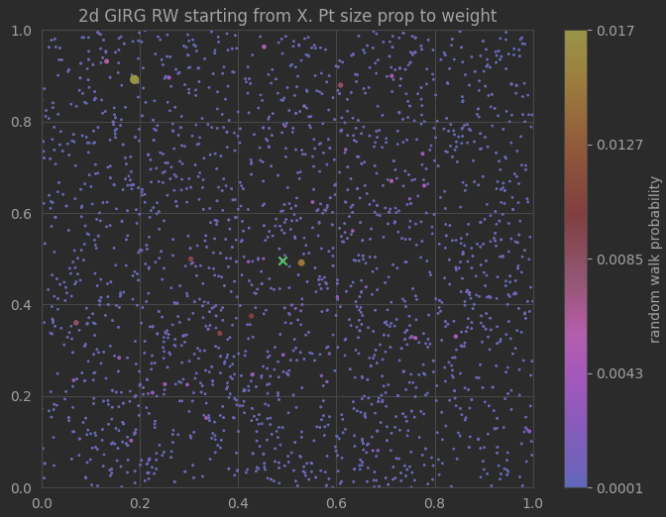
\includegraphics[width=\linewidth]{figures/2d_GIRG_RW.png}
    \caption{Naive edge weightings: Large weight nodes get disproportionately more probability mass.}
  \end{subfigure}
  \hfill
  \begin{subfigure}{0.49\textwidth}
    \centering
    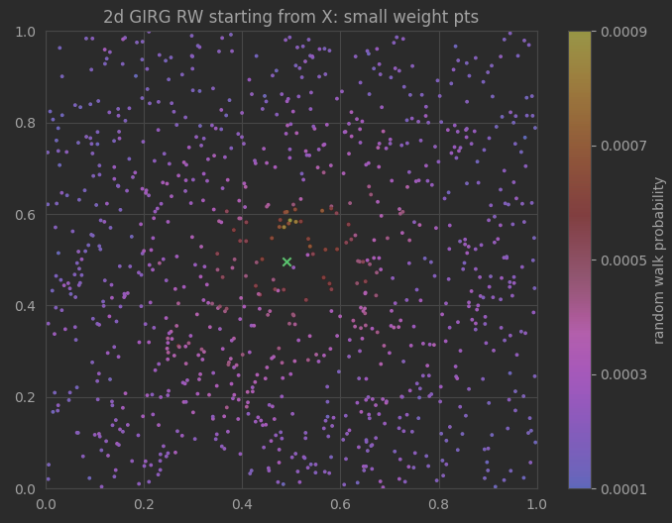
\includegraphics[width=\linewidth]{figures/2d_GIRG_RW_small_weights.png}
    \caption{Restriction of Naive approach plot to nodes with smaller weights. Probability distribution looks more gaussian}
  \end{subfigure}

  \vspace{1em}

  \begin{subfigure}{0.49\textwidth}
    \centering
    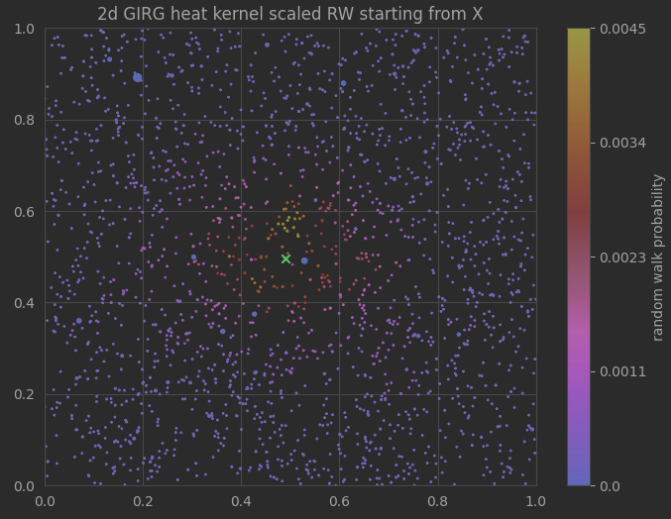
\includegraphics[width=\linewidth]{figures/2d_GIRG_heatkernelscaled_RW.png}
    \caption{Heat Kernel expected edge distance scaled edge weights $W_{uv} = e^{-\hat{r}_{uv}^2}$. Helps to remove the large weight bias - perhaps too much as large weight nodes are too cold.}
  \end{subfigure}
  \hfill
  \begin{subfigure}{0.49\textwidth}
    \centering
    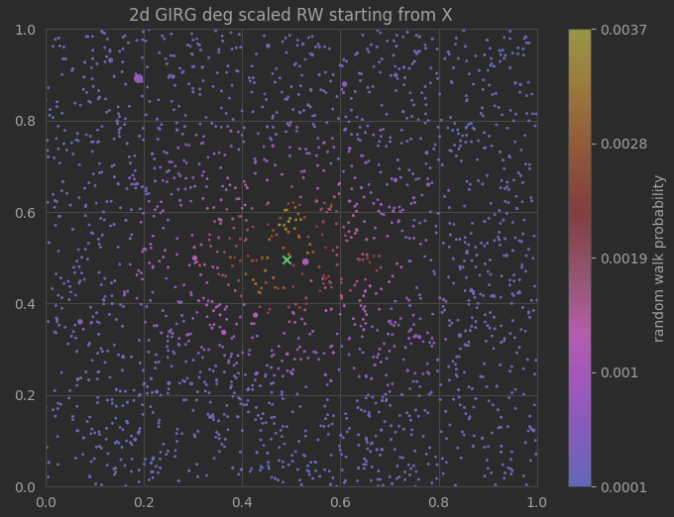
\includegraphics[width=\linewidth]{figures/2d_GIRG_degscaled_RW.png}
    \caption{Homogeneous approach scaling edge weights by node degree $d_i^{-1}$  also removes the large weight bias, seemingly more evenly}
    \label{fig:diffmap_algo_comparisons_degscaled}
  \end{subfigure}
  \caption{$t=6$ step random walk diffusion cloud on a 2d torus GIRG. Each point is a node shown at its location $\vec{x}_u \in [0, 1]^2$. $u_{t=0}$ is the node marked with the green x. Point colour denotes probability mass in the diffusion cloud.Point radius is proportional to node weight $w_u$. Three different random walks are shown corresponding to our three different graph edge weighting (transition probability) schemes.}
  \label{fig:diffmap_algo_comparisons}
  % \caption{Diffusion map eigenvalues (including $\lambda_1 = 1$) for a $n=2000, \tau=2.5, \alpha=1.3$ Cube GIRG with $d=1,2,3,4$ dimensions.}
  % \label{fig:cube_diffmaps_d1to4_evals}
\end{figure}



% % 
% The m-truncated diffusion map representation becomes the new r epresentation of nodes in the graph. The diffusion map is then a function $\R^n \to \R^m$. The first coordinate $\lambda_1$ is always $1$, corresponding to the stationary distribution of the random walk which all node diffusion maps converge to. This is useless for differentiating nodes and is hence dropped.

% Notably the transition matrix satisfies $M1 = 1$ since $\sum_j \frac{w_{ij}}{\deg(i)} = 1$, and it can be shown that it has eigenvalues $\lambda_1=1 \geq \lambda_2 \geq \lambda_3 \geq ...$.  





% Oh no $\vec{x}$.

% by the transition matrix $M = D^{-1}W$, where $D$ is the diagonal matrix with $D_{uu} = \sum_{v\in V} W_{uv}$ is the diagonal degree matrix, and $W_{uv}$ is the adjacency matrix, $W_{uv} = \begin{cases}1 & u \sim v \\0 & u \nsim v \end{cases}$. The matrix $S = D^{-1/2} W D^{-1/2}$ is a symmetrised version and hence is diagonalisable as $S = V \Lambda V^T$. Then the map $M = D^{-1/2} S D^{1/2} = D^{-1/2} V \Lambda (D^{1/2} V)^T = \Phi \Lambda \Psi^T$.

% In particular, starting at node $i$ (numbered $i=1,...,n$), the $t$th step diffusion cloud is $i \mapsto M^t_{ij} = (\Phi \Lambda^t \Psi^T)_{ij} = \sum_{k=1}^n \Phi_{ik} \lambda_k^t \Psi_{jk}$.

% So writing $\Phi = [\phi_1, \phi_2, ..., \phi_n]$ and $\Psi = [\psi_1, \psi_2, ..., \psi_n]$, we have that the $t$th step diffusion cloud is $i \mapsto \sum_{k=1}^n \phi_k(i) \lambda_k^t \vec{\psi}_k$. I.e. the diffusion map coordinate system is $\text{diffmap}_t(i) = (\lambda_2^t \phi_2(i), \lambda_3^t \phi_3(i), ..., \lambda_{d+1}^t \phi_{d+1}(i))$. The first coordinate is always $1$, it's the stationary distribution that all diffusion clouds converge to, so is discarded.

\section{Empirical Results and Post-Processing}
We see in \cref{fig:cube_diffmap_plots_d1and2} some 2d truncated diffusion maps. When the underlying graph was a 2d cube GIRG, the inferred points indeed look square like. From the 1d GIRG we get a curved line shape - i.e. a 1d manifold embedded in 2d, as expected. In testing diffusion maps on max norm torus / cube geometries, replication of node locations was very good. We additionally tested distorted GIRG variants to see if atenuating the signal of some dimensions would monotonically degenerate their diffusion map embedding - this was observed to be the case. We did not test diffusion maps on MCD GIRGs, though this would be interesting. We think in theory that, although the brownian motion would look unusual, no longer euclidean geometry like, the diffusion map embedding should still be able to recover the original geometry. This would be good to test in future work. 

We detail some post processing steps that can be done to improve diffusion map embedding for both GIRG generated graphs, and real graphs (real graphs in particular produce wilder diffusion maps due to their idiosyncratic connectivity patterns).

\begin{figure}
  \centering

  \begin{subfigure}{0.49\textwidth}
    \centering
    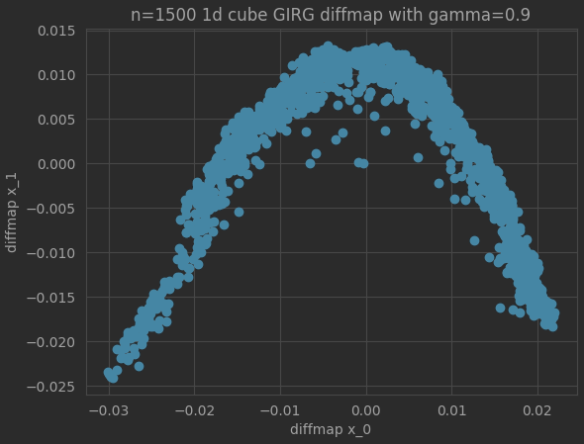
\includegraphics[width=\linewidth]{figures/1d_GIRG_diffmap.png}
    \caption{1d cube GIRG 2d diff map}
    \label{fig:sub1}
  \end{subfigure}
  \hfill
  \begin{subfigure}{0.49\textwidth}
    \centering
    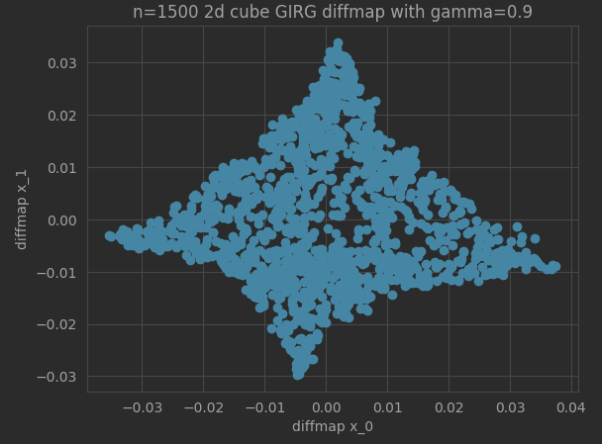
\includegraphics[width=\linewidth]{figures/2d_GIRG_diffmap.png}
    \caption{2d cube GIRG 2d diff map}
    \label{fig:cube_diffmap_plots_d2}
  \end{subfigure}


  \caption{Diffusion map scatter plot of the 2d truncated diffusion maps of (a) graph from a 1d cube GIRG, (b) graph from a 2d cube GIRG. Each plotted point is the inferred location of a single node. }
  \label{fig:cube_diffmap_plots_d1and2}
\end{figure}

\subsection{Inferring Dimension $d$}
If we have a graph $G$ which we know is generated from a $d$-dimensional GIRG, we can simply extract the $d$-truncated diffusion map coordinates of each node as an initial estimate for the original geometric location of the node. 

However if the true geometric dimension $d$ is unknown, an important first question is how to choose the output dimension $d$ (truncation for the embedding) of the diffusion map.

Diffusion maps actually present one way to infer the dimensionality by analysing the ordered sequence of eigenvalues $\lambda_2 < \lambda_3 < ...$. For example in \cref{fig:cube_diffmaps_d1to4_evals} we see that for graphs generated from cube GIRGs with dimension $d=1,2,3,4$, the diffusion map eigenvalue have a clear cutoff point after the first $d+1$ eigenvalues, with $\lambda_2, ..., \lambda_{d+1}$ being all approximately equal. Hence an eigenvalue cutoff can be used to infer geometric dimensionality of a graph. This is inherently manual/empirical, and so more difficult for real world graphs.

\paragraph{Toroidal GIRGs diffusion map eigenvalues} Interestingly Toroidal GIRGs are differentiated from Cube GIRGs in that the diffusion map requires $2d$ coordinates to capture the Torus geometry instead of just $d$ for the cube. The natural diffusion map of a 1D Torus GIRG ends up being a 2d circle about the origin; 2 large eigenvalues $\lambda_2, \lambda_3$ are necessary. This representation of the torus does accurately retain interpoint distances which is what we care for the most, however if you really knew that it was a torus of some dimension, you could project the embedding back into the torus space for a more compact representation. For instance \cite{garcia2019mercator} map 2d points to an angle of direction away from the origin $\phi \in [0, 2\pi)$ using arctan.

% TODO plot some real graph eigenvalue plots?

% If there is a good cutoff point whereby the first $d$ eigenvalues are of similar large size, and the rest are much smaller, . This indeed works well for graphs synthetically generated from GIRGs, not so well on real world graphs.



\begin{figure}
  \centering

  \begin{subfigure}{0.45\textwidth}
    \centering
    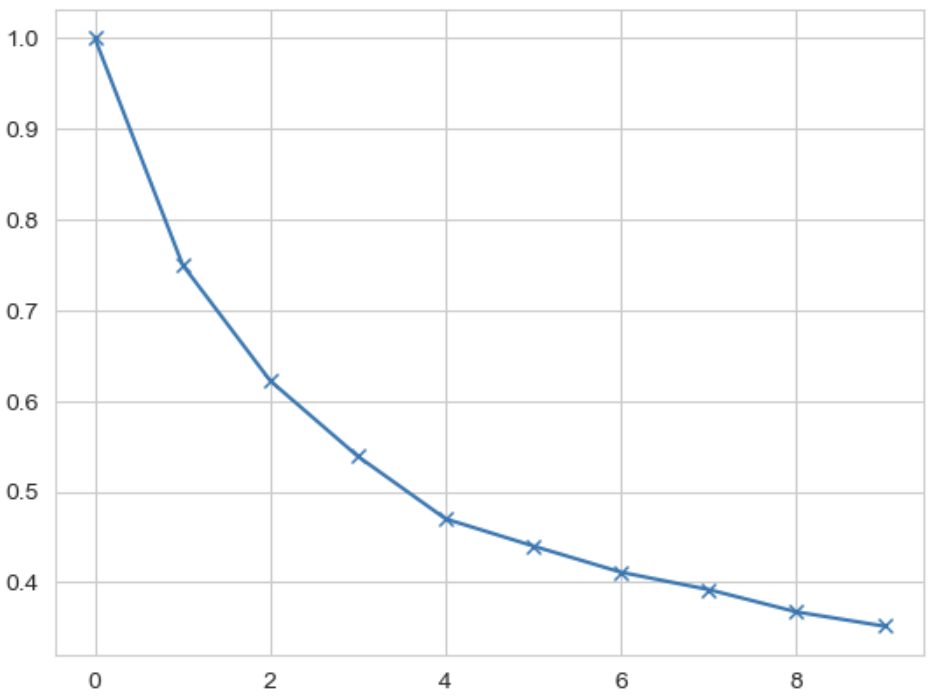
\includegraphics[width=\linewidth]{figures/diffmap_1d.png}
    \caption{$d=1$}
  \end{subfigure}
  \hfill
  \begin{subfigure}{0.45\textwidth}
    \centering
    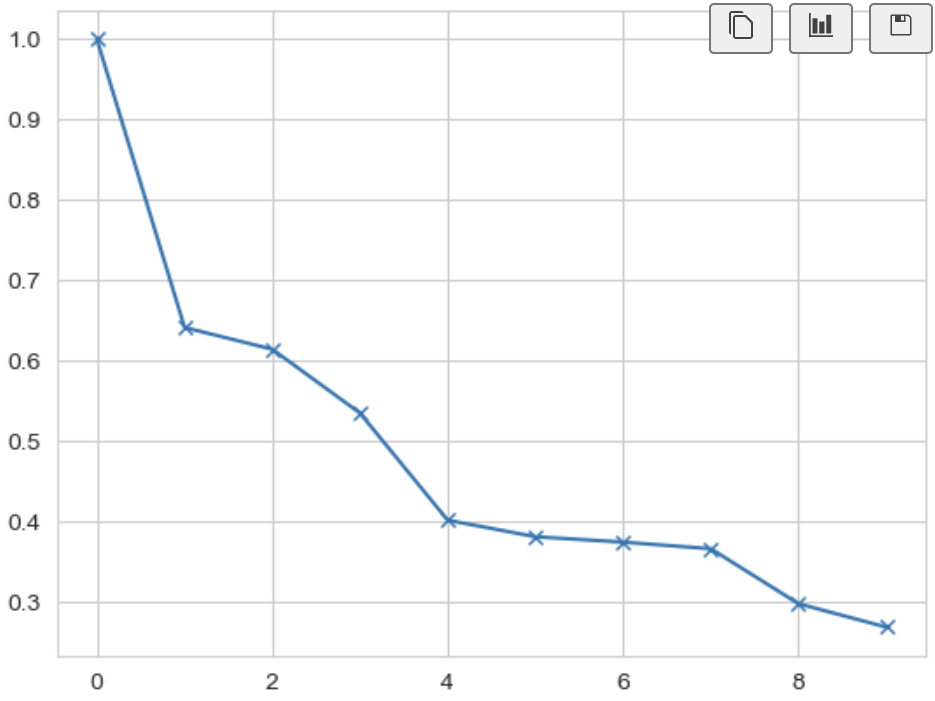
\includegraphics[width=\linewidth]{figures/diffmap_2d.png}
    \caption{$d=2$}
  \end{subfigure}

  \vspace{1em}

  \begin{subfigure}{0.45\textwidth}
    \centering
    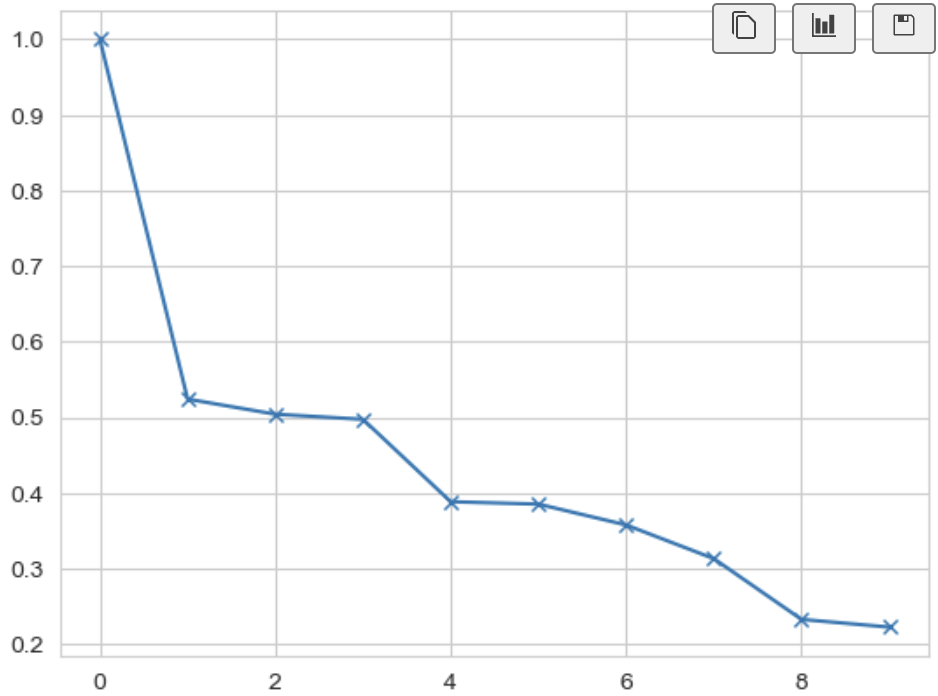
\includegraphics[width=\linewidth]{figures/diffmap_3d.png}
    \caption{$d=3$}
  \end{subfigure}
  \hfill
  \begin{subfigure}{0.45\textwidth}
    \centering
    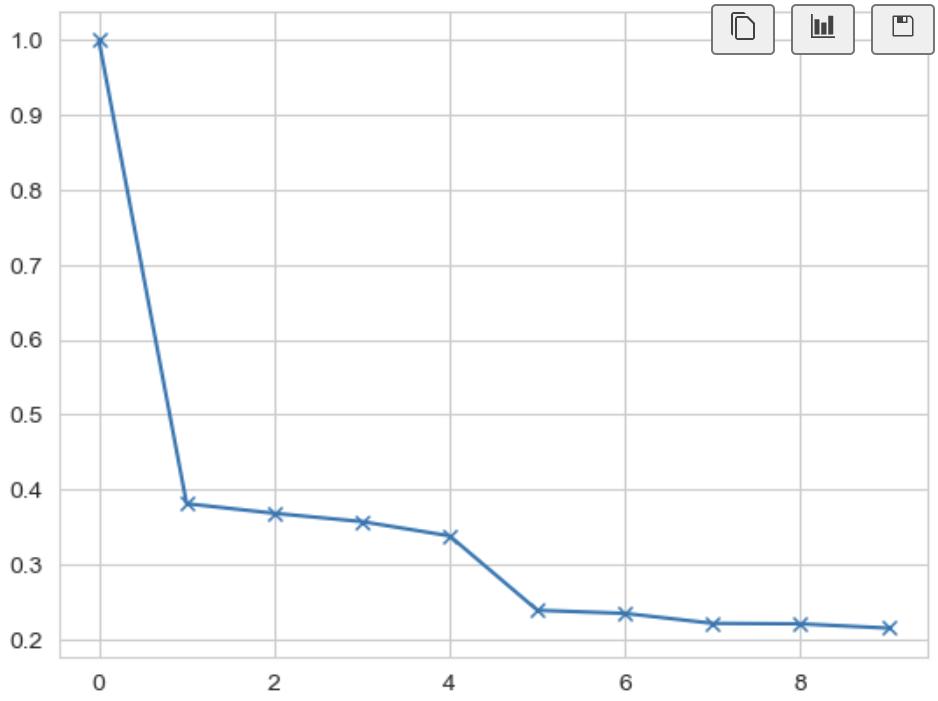
\includegraphics[width=\linewidth]{figures/diffmap_4d.png}
    \caption{$d=4$}
    \label{fig:cube_diffmaps_d4}
  \end{subfigure}

  \caption{Eigenvalues of the diffusion map laplacian matrix (including $\lambda_1 = 1$) for 4 different $n=2000, \tau=2.5, \alpha=1.3$ cube GIRGs: with dimensions $d=1,2,3,4$. X-axis is the ith eigenvalue, y-axis is the eigenvalue value.}
  \label{fig:cube_diffmaps_d1to4_evals}
\end{figure}

\subsection{Rescaling/Shifting Diffusion Maps}
From \cref{sec:diff_map_geometry} we know that the diffusion map embeddings should be roughly isometric up to a scale factor - so rescaling and shifting into the unit cube/torus is important to make inter-point distances meaningful/consistent across multiple graphs (even though this could be absorbed into the probability scaling constant $c$).


The embeddings will be centered around the origin, as all $\lambda_2, \lambda_3, ...$ eigenvalue eigenvectors are orthogonal to $\vec{\phi}_1 = k \vec{1}$ : they represent a deviation from the stationary distribution. E.g. in a 1d cube GIRG for a node with $\vec{x}_u \approxeq 0$ at the extreme geometric left end, its diffusion cloud will need to put more diffusion probability on the left side nodes and less on the right side nodes than the stationary distribution.


In order to map embeddings into the $[0, 1]^d$ torus/cube, the 0 centering can easily be fixed by shifting the points $(\vec{x}_u)_i \gets (\vec{x}_u)_i + \min_v (\vec{x}_v)_i$.
If we are certain that the points should be distributed within the unit cube, then we can simply rescale separately along each dimension: $x \gets \frac{x - x_{\min}}{x_{\max} - x_{\min}}$.
If furthermore we're certain that the distribution within the unit cube should be relatively uniform, we can perform a coordinatewise $\uniformify$ procedure that replaces $(\vec{x}_u)_i$ with its percentile value compared with other $(\vec{x}_v)_i$. \cref{fig:diffmap_uniformed_vs_nonuniformed} shows the $\uniformify$ procedure in action.
Real graphs' diffusion maps are often quite non-uniformly located points, with some highly bunched up and others spread out, so $\uniformify$ can be quite useful in this case.

% helps to counteract the phenomenon of terribly different diffusion map scaling, whereby the majority of the graph which is well connected ends up highly bunched up, and a small number of outlying poorly connected nodes cover most of the embedding space. 

% Notably on real graphs where the truncated diff map coordinates are not guaranteed to be independently distributed, coordinatewise percentile mapping can lead to slightly odd results - see socfb-Amherst where there's a strong $x_1 = 1 - x_2$ correlation for small $x_1$. It's still a good improvement over the original non rescaled diffusion map.

% The decreasing diffusion map scaling can be see either as a bug or a feature. If we are certain that the points should be distributed within the unit cube, then we can simply rescale separately along each dimension: $x \gets \frac{x - x_{\min}}{x_{\max} - x_{\min}}$. If furthermore we're certain that the distribution within the unit cube should be relatively uniform, we can perform a coordinatewise "uniformify" procedure that replaces $(x_u)_i$ with its percentile value compared with other $(x_v)_i$. \cref{fig:diffmap_uniformed_vs_nonuniformed} shows the "uniformify" procedure in action. Notably on real graphs where the truncated diff map coordinates are not guaranteed to be independently distributed, coordinatewise percentile mapping can lead to slightly odd results - see socfb-Amherst where there's a strong $x_1 = 1 - x_2$ correlation for small $x_1$. It's still a good improvement over the original non rescaled diffusion map. 

% Critically since there is no guarantee that the scaling of diffusion map coordinates is the same as the original GIRG coordinates, using some kind of prior knowledge to rescale the diffusion map is important to yield geometric information with meaningful inter-point distances.

\begin{figure}
  \centering

  \begin{subfigure}{0.49\textwidth}
    \centering
    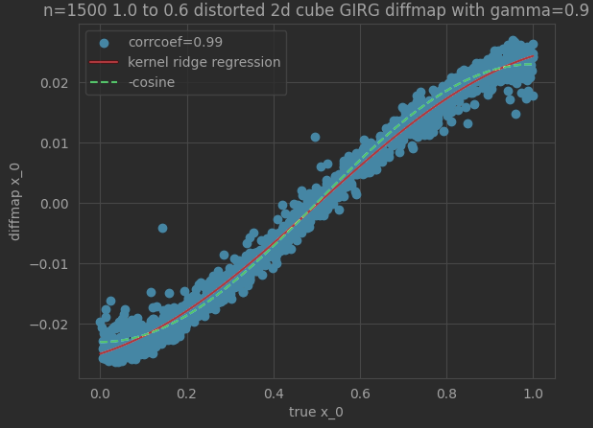
\includegraphics[width=\linewidth]{figures/2d_distorted_diffmap_plot_major.png}
    \caption{First dimension - larger weight scaling in distance function. As the more geometry influencing dimension, it is easier for the diffusion map to fit well, and is picked up as the largest non $1$ eigenvalue. The fit is quite close to a cosine wave as shown.}
    \label{fig:2d_distorted_major}
  \end{subfigure}
  \hfill
  \begin{subfigure}{0.49\textwidth}
    \centering
    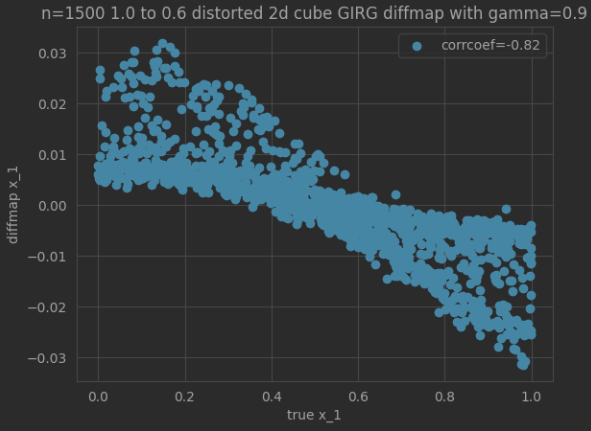
\includegraphics[width=\linewidth]{figures/2d_distorted_diffmap_plot_minor.png}
    \caption{Second (minor) dimension - diffusion map has more trouble fitting this information as it is harder to distinguish from noise. Note a linear relationship means success - negative gradient is irrelevant.}
    \label{fig:2d_distorted_minor}
  \end{subfigure}


  \caption{2d distorted cube GIRG. 2 dim truncated diffusion map embeddings shown with one plot for each dimension. Each plotted point is one node from the graph, with X-axis being its true location in the 2d cube for that dimension, and Y-axis being the diffusion map embedding.}
  \label{fig:2d_distorted_major_minor}
\end{figure}


\paragraph{Rotated Points} One issue with diffusion maps as seen in \cref{fig:cube_diffmap_plots_d2} is rotations - the 2d GIRG's points are rotated into a diamond shape. As we only hope for an isometric mapping of the original point locations to the diffusion map embedding, we can't expect the diffusion map embedding to be in the same basis as the original point locations. If we want to fit it back into $[0, 1]^d$, we don't care about reflections, and we can translate and rescale, however rotating is more difficult.

That \cref{fig:cube_diffmap_plots_d2} looks almost perfectly 45 degree rotated could potentially be explained as the diffusion map trying to maximise diffusion explainability - the long square diagonal has overall more diffusion along it so might be picked up as a major eigenvalue - maybe a small imbalance of more nodes in one corner can cause this. Even assuming no overall rotation bias, you're going to get a square rotated somewhere between $0$ and $45$ degrees.

\paragraph{Distorted GIRGs make cuboidal diffusion map embeddings} In practice, real graphs never have a perfectly equal balance in geometric dimension importance. 
We introduced distorted GIRGs in \cref{subsec:distorted_girgs} as a possible model for this, where for example the distance function could be the weighted Euclidean norm in 2d: $\norm{x - y}^2 = a (x_1 - y_1)^2 + b(x_2 - y_2)^2$. If $a > b$, even just by a little amount, then the first diffusion map coordinate $\varphi_1(u)$ is likely to be very similar to $(\vec{x}_u)_1$. Only if $a=b$ is there no preference between $(\vec{x}_u)_1$ and $(\vec{x}_u)_2$, making a rotation possible.
Hence the points $(\varphi_1(u), \varphi_2(u))_{u \in V}$ are likely to end up as a rectangle, not a rotated square; the variation in first coordinate will be greater than in the second.

\cref{fig:2d_distorted_major} shows the 2d diff map embedding of such a distorted 2d cube GIRG. Note that the major coordinate is much easier to fit well, whereas the minor one has higher error (NB the diff map embedding of $x_2$ is negatively scaling with the true value which is fine - we can never guarantee same signs).
We also see that the $x_1$ diffusion map embedding does not have quite a linear relationship with the real locations - it looks more like a cosin wave like relationship - this actually makes sense as eigenfunctions of the laplacian operator on a cube look like sin waves.


In the light of potentially non equal coordinates, the relative $\lambda_2 > \lambda_3 > ...$ scaling can be seen as a feature not a bug, if the hypothesis space of generative graph models is to be expanded to cuboid (non-cube) GIRGs. In this case all coordinates of the diffusion map don't have to be all (non-homogeneously) rescaled to the range $[0, 1]$ and can rather be homogeneously rescaled to retain their relative size ratios.
This sheds new light on the horizontalness of the $\lambda_2, \lambda_3, \lambda_4, \lambda_5$ line segment in \cref{fig:cube_diffmaps_d4} as a testament to the underlying cubeness (non cuboid) of the GIRG that generated the graph.




% In this case, the diffusion map coordinates will have a larger scale for the $\lambda_2$ coordinate than the $\lambda_3$ coordinate, and the points will look like an elongated rectangle.

% the distance: $\norm{x - y} = \sqrt{a (x_1 - y_1)^2 + b(x_2 - y_2)^2}$. In this case, the diffusion map coordinates will have a larger scale for the $\lambda_2$ coordinate than the $\lambda_3$ coordinate, and the points will look like an elongated rectangle. The flatness of $\lambda_2, \lambda_3, \lambda_4, \lambda_5$ line segment in \cref{fig:cube_diffmaps_d4} is a testament to the cube (and non cuboidness) of the underlying GIRG that generated the graph.


% (relatively uniformly) distributed within the unit cube, then we can simply rescale separately along each dimension.
% A linear coordinatewise scaling $x \gets \frac{x - x_{\min}}{x_{\max} - x_{\min}}$ works, or more extremely a coordinatewise "uniformify" procedure that replaces $(x_u)_i$ with its percentile value compared with other $(x_v)_i$.
% In \cref{fig:diffmap_uniformed_vs_nonuniformed} we see uniformified versions of a generated 2D GIRG, and the socfb-Amherst41 graph.

% Seen as a feature, the relatively different scaling allows as a natural correction to the potential non equivalence of different dimensions. For instance in a weighted euclidean norm setup, it could be that a 2D GIRG's true 1st geometric dimension (between $[0, 1]$) is much more important than its 2nd geometric dimension in determining the distance: $\norm{x - y} = \sqrt{a (x_1 - y_1)^2 + b(x_2 - y_2)^2}$. In this case, the diffusion map coordinates will have a larger scale for the $\lambda_2$ coordinate than the $\lambda_3$ coordinate, and the points will look like an elongated rectangle. The flatness of $\lambda_2, \lambda_3, \lambda_4, \lambda_5$ line segment in \cref{fig:cube_diffmaps_d4} is a testament to the cube (and non cuboidness) of the underlying GIRG that generated the graph. 


% TODO put in some eigenvalue plots


\begin{figure}
    \centering

    \begin{subfigure}{0.45\textwidth}
      \centering
      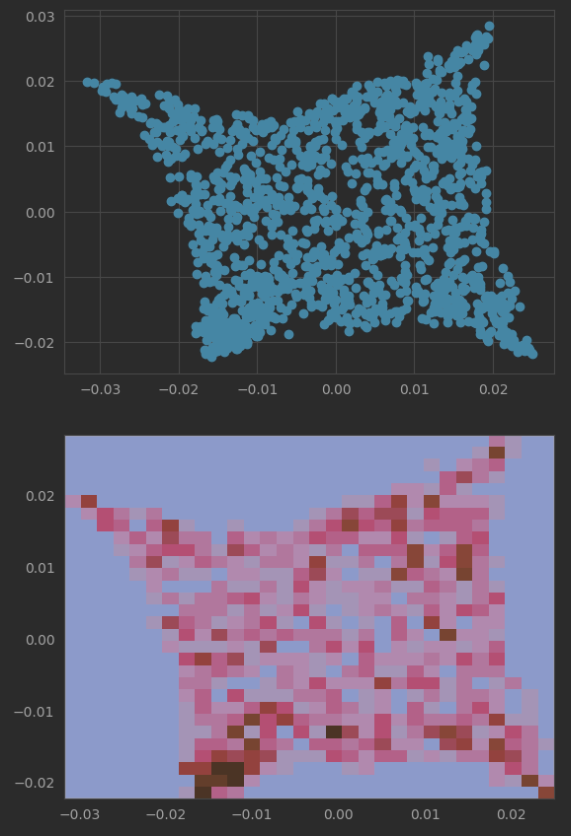
\includegraphics[width=\linewidth]{figures/diffmap_plot_nonuniformed.png}
      \caption{2d cube GIRG diff map}
      \label{fig:sub1}
    \end{subfigure}
    \hfill
    \begin{subfigure}{0.45\textwidth}
      \centering
      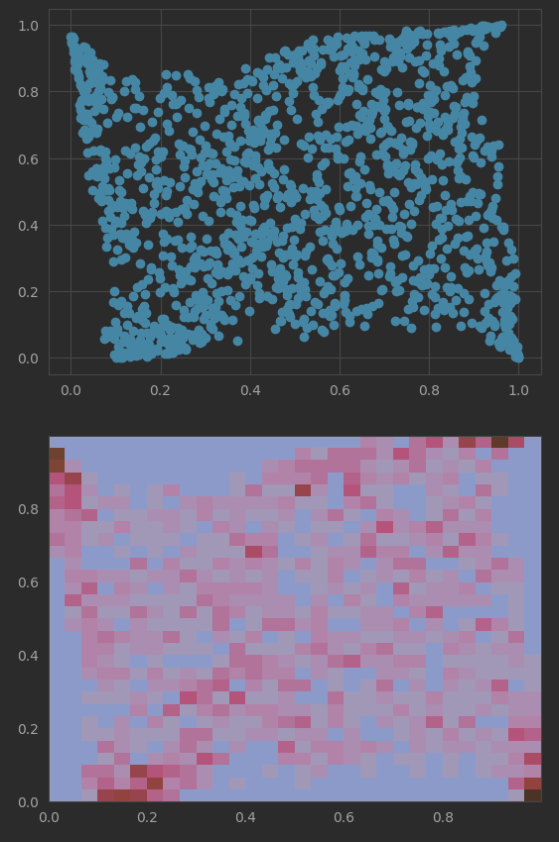
\includegraphics[width=\linewidth]{figures/diffmap_plot_uniformed.png}
      \caption{2d cube GIRG diff map with $\uniformify$ rescaling}
      \label{fig:sub2}
    \end{subfigure}
  
    \vspace{1em}
  
    \begin{subfigure}{0.45\textwidth}
      \centering
      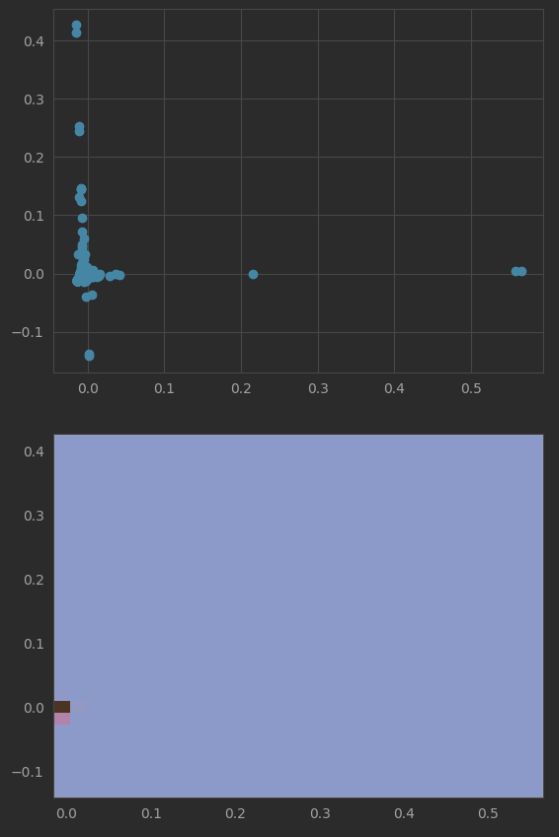
\includegraphics[width=\linewidth]{figures/real_diffmap_plot_nonuniformed.png}
      \caption{socfb-Amherst41 diff map}
      \label{fig:sub3}
    \end{subfigure}
    \hfill
    \begin{subfigure}{0.45\textwidth}
      \centering
      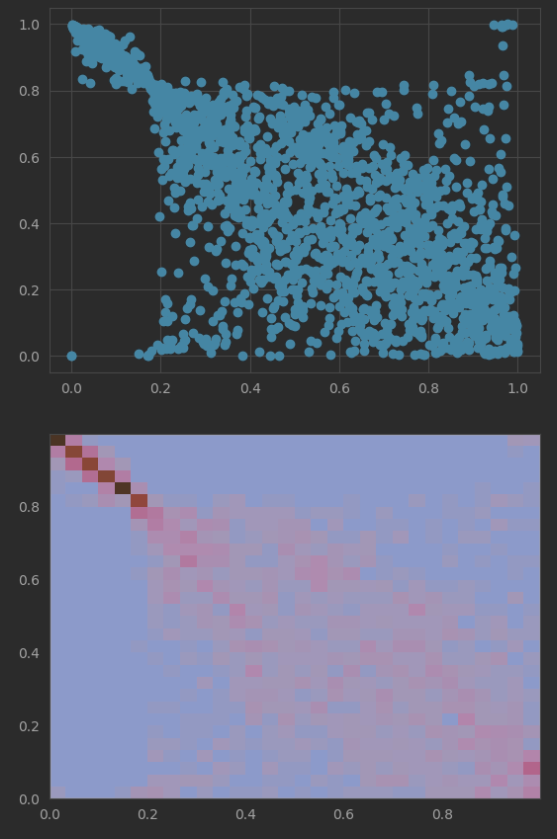
\includegraphics[width=\linewidth]{figures/real_diffmap_plot_uniformed.png}
      \caption{socfb-Amherst41 diff map with $\uniformify$ rescaling}
      \label{fig:sub4}
    \end{subfigure}
    \caption{
      2d truncated diffusion maps plotted - each point is the embedding of a node in the graph. (a) and (b) are on a 2d GIRG, (c) and (d) on a real-world social network graph. The affect of the $\uniformify$ point rescaling procedure is shown, in (b) and (d).}
    \label{fig:diffmap_uniformed_vs_nonuniformed}
\end{figure}


% \begin{figure}
%   \centering

%   \begin{subfigure}{\textwidth}
%     \centering
%     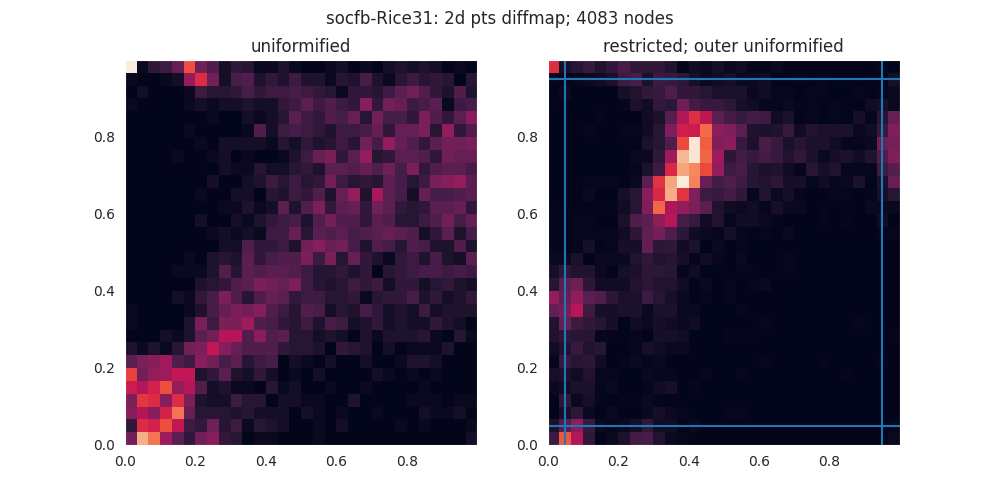
\includegraphics[width=\linewidth]{figures/socfb-Rice31_2ddiffmap_unif_vs_restrict.png}
%     % \label{fig:sub1}
%   \end{subfigure}

%   \vspace{1em}
%   \begin{subfigure}{\textwidth}
%     \centering
%     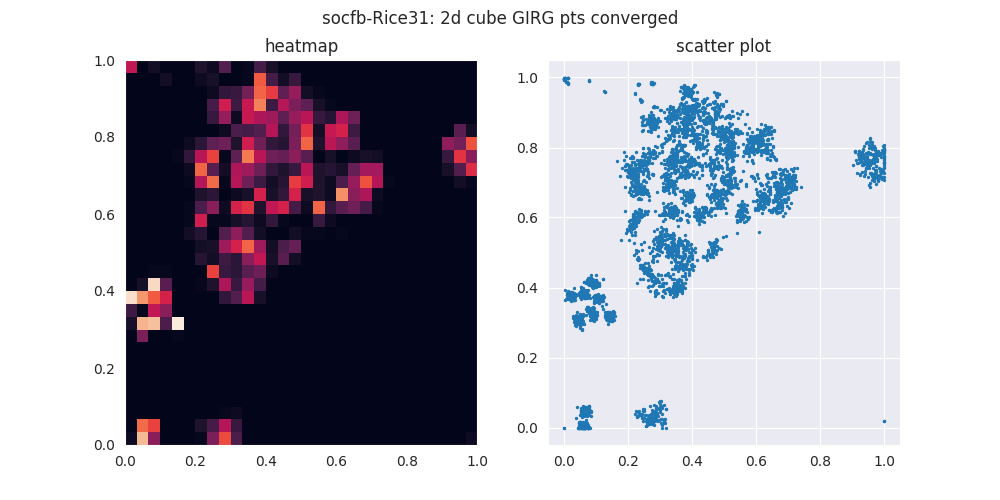
\includegraphics[width=\linewidth]{figures/socfb-Rice31_2d_cube_GIRG_converged.png}
%     % \label{fig:sub1}
%   \end{subfigure}

%   \vspace{1em}
  
% \end{figure}
% \begin{figure}
%   \begin{subfigure}{\textwidth}
%     \centering
%     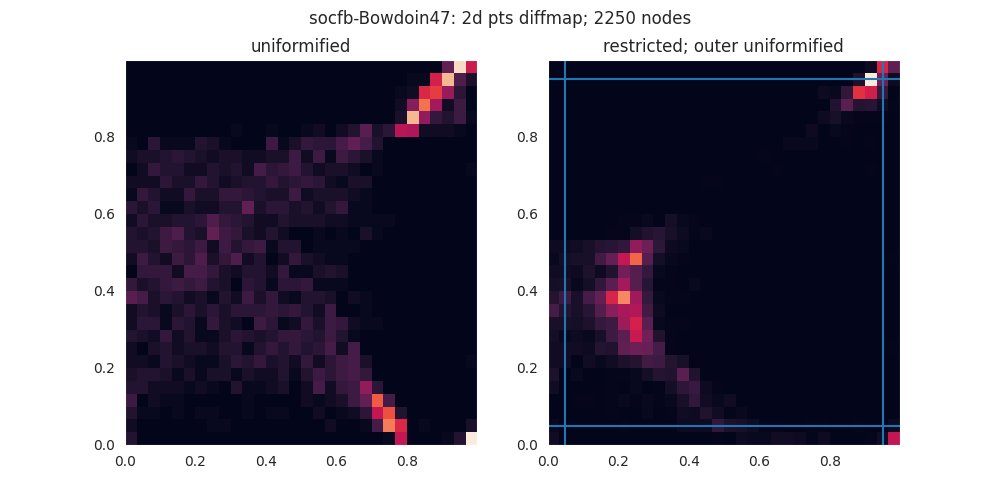
\includegraphics[width=\linewidth]{figures/socfb-Bowdoin47_2ddiffmap_unif_vs_restrict.png}
%     % \label{fig:sub1}
%   \end{subfigure}

%   \vspace{1em}
%   \begin{subfigure}{\textwidth}
%     \centering
%     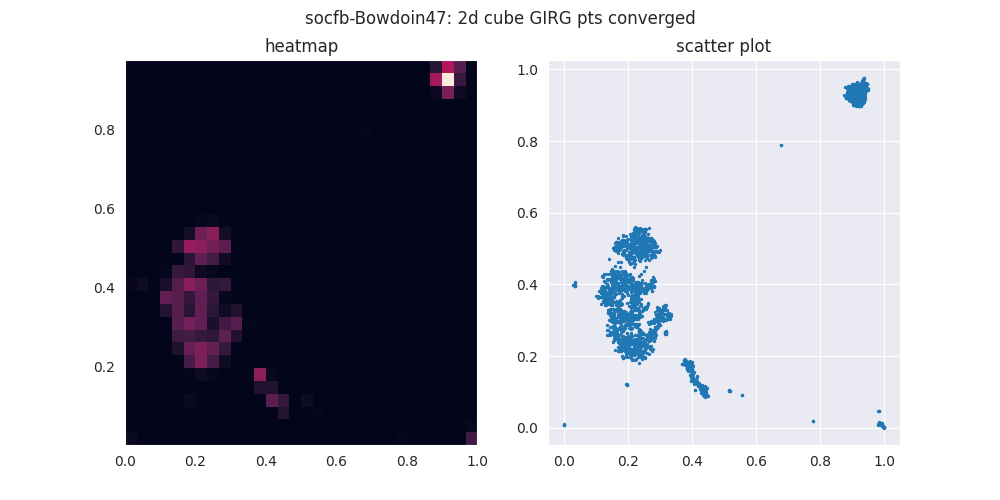
\includegraphics[width=\linewidth]{figures/socfb-Bowdoin47_2d_cube_GIRG_converged.png}
%     % \label{fig:sub1}
%   \end{subfigure}

% \end{figure}


% \begin{figure}
%   \begin{subfigure}{\textwidth}
%     \centering
%     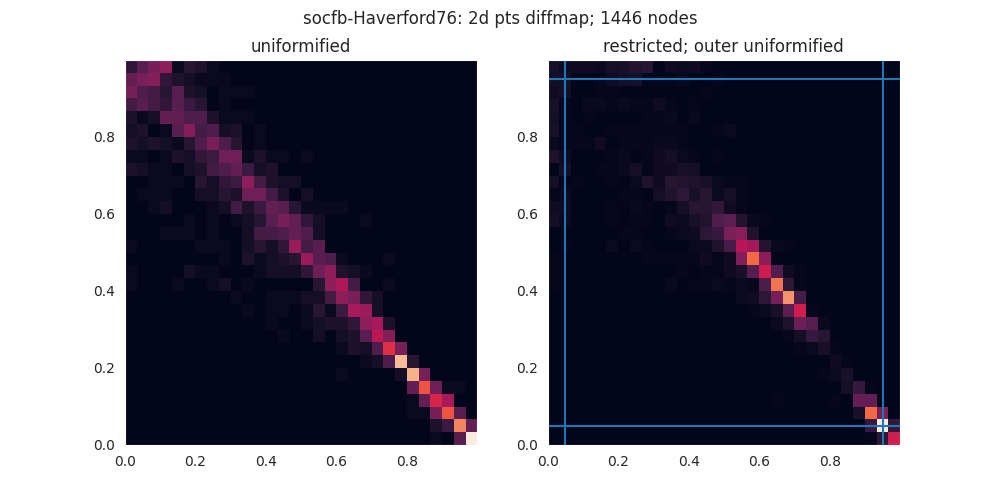
\includegraphics[width=\linewidth]{figures/socfb-Haverford76_2ddiffmap_unif_vs_restrict.png}
%     % \label{fig:sub1}
%   \end{subfigure}

%   \vspace{1em}
%   \begin{subfigure}{\textwidth}
%     \centering
%     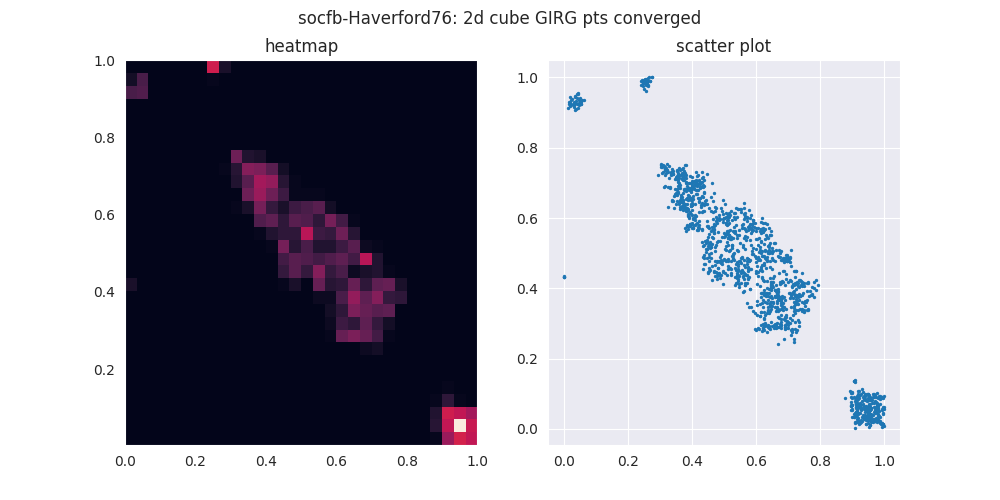
\includegraphics[width=\linewidth]{figures/socfb-Haverford76_2d_cube_GIRG_converged.png}
%     % \label{fig:sub1}
%   \end{subfigure}


%   \caption{two methods for rescaling/shifting diffusion maps into the cube - done here for d=2 truncations. The blue lines for the restricted version show the border at which points are outer uniformified.}
%   \label{fig:uniformifed_vs_restricted_rescaling}
% \end{figure}



% A final issue with diffusion maps is that points seem to end up concentrated in corners/edges. My hypothesis is that this is because e.g. on a 1D line segment, it's hard to distinguish somewhat left and very left points - in the end the diffusion cloud bias is still just left leaning. Not sure how much of a problem this is.

\paragraph{Restricted Rescaling} This simple post processing method aims to map points into a reasonable geometric space without strongly biasing towards a uniformly distributed prior like the $\uniformify$ procedure.
Empirically, the diffusion map coordinates of real-world facebook graphs often have $\geq 90\%$ of the nodes concentrated in a small parcel, with only a few nodes having extremely far out locations. This is due to most nodes being very well interconnected, and some being much more torturously linked to the central hub - hence ending up with great diffusion distance separation.
This defeats the simple rescaling method of $x \gets \frac{x - x_{\min}}{x_{\max} - x_{\min}}$ as most nodes will end up very tightly packed. However if we hit all the points with the $\uniformify$ procedure hammer, we might lose some of the subtleties of the geometry picked up by the diffusion map within the highly connected central parcel.

Instead we only rescale the central nodes: those whose joint coordinate-wise percentiles lie in $[5\%, 95\%]^d$; they are linearly scaled to the $[0.05, 0.95]^d$ cube. Finally the outlying nodes are percentile rescaled (non-linearly) to the upper/lower cube margins.
This method is shown in comparison for a few graphs in \cref{fig:uniformifed_vs_restricted_rescaling}


% \begin{figure}
%   \begin{subfigure}{0.47\textwidth}
%     \centering
%     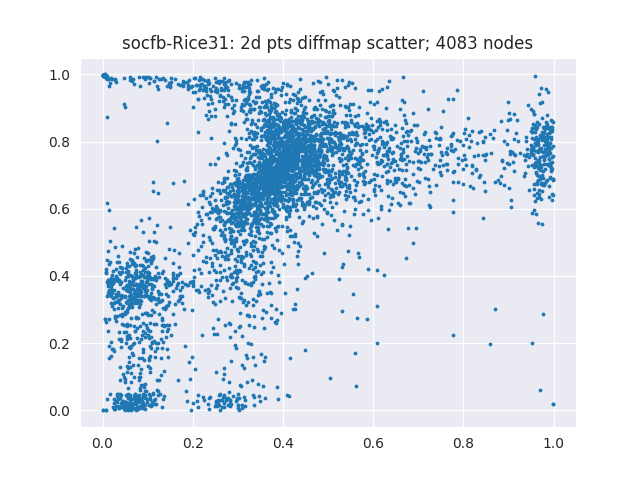
\includegraphics[width=\linewidth]{figures/socfb-Rice31_2ddiffmap_restrict_scatter.png}
%     % \label{fig:sub1}
%   \end{subfigure}
%   \hfill
%   \begin{subfigure}{0.47\textwidth}
%     \centering
%     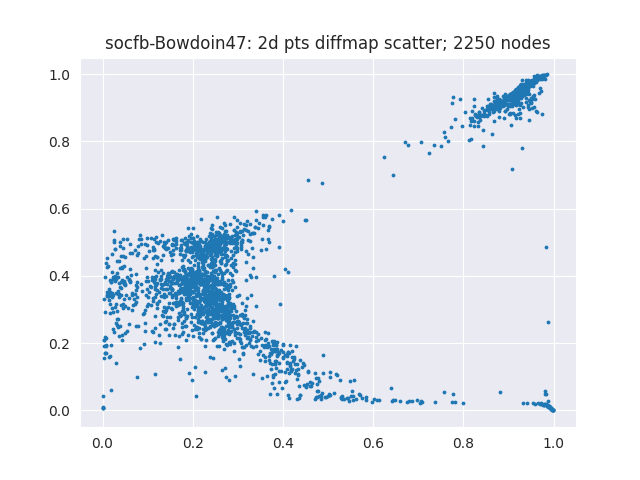
\includegraphics[width=\linewidth]{figures/socfb-Bowdoin47_2ddiffmap_restrict_scatter.png}
%     % \label{fig:sub1}
%   \end{subfigure}
%   \caption{the diffmaps (here 2d, restricted and outer uniformified) don't have much point clustering - it's more higher diffusion level than caring so much about individual edges like in the converged case}
%   \label{fig:uniformifed_vs_restricted_rescaling}
% \end{figure}

% TODO 

% - fuller analysis of different diffmap modes: 'uniformify', 'cubify' and 'cuboidify', comparing performance on real life and synthetic graphs

% - presentation of the small degree stochastic walk tweak which improves diffusion map performance:
% \begin{verbatim}
% # Empirically this gamma seems to work well. 
% # It discourages taking edges to popular nhbs.
% gamma = 0.9
% M_tilde = scipy.sparse.diags(1 / D) @ A @ scipy.sparse.diags(D ** (-gamma))
% M_tilde = scipy.sparse.diags(np.array(1 / M_tilde.sum(axis=-1)).squeeze()) @ M_tild
% \end{verbatim}

% - is it true that diffusion map tends to cluster representations edges rather than being more uniform? Empricially seems to happen in 2D but not 1D?

